%package list
\documentclass{article}
\usepackage[top=3cm, bottom=3cm, outer=3cm, inner=3cm]{geometry}
\usepackage{graphicx}
\usepackage{url}

%% \usepackage{cite}
\usepackage{hyperref}
\usepackage{array}
\usepackage{multicol}
\newcolumntype{x}[1]{>{\centering\arraybackslash\hspace{0pt}}p{#1}}
\usepackage{natbib}
\usepackage{pdfpages}
\usepackage{multirow}
\usepackage{float}
\usepackage[normalem]{ulem}
\useunder{\uline}{\ul}{}


%%%%%%%%%%%%%%%%%%%%%%%%%%%%%%%%%%%%%%%%%%%%%%%%%%%%%%%%%%%%%%%%%%%%%%%%%%%%
%%%%%%%%%%%%%%%%%%%%%%%%%%%%%%%%%%%%%%%%%%%%%%%%%%%%%%%%%%%%%%%%%%%%%%%%%%%%
\newcommand{\csemail}{vmachacaa@unsa.edu.pe}
\newcommand{\csdocente}{Vicente Machaca Arceda}
\newcommand{\cscurso}{Algoritmos y Estructura de Datos}
\newcommand{\csuniversidad}{Universidad Nacional de San Agustín}
\newcommand{\csescuela}{Maestría en Ciencia de la Computación}
\newcommand{\cspracnr}{04}
\newcommand{\cstema}{--}
%%%%%%%%%%%%%%%%%%%%%%%%%%%%%%%%%%%%%%%%%%%%%%%%%%%%%%%%%%%%%%%%%%%%%%%%%%%%
%%%%%%%%%%%%%%%%%%%%%%%%%%%%%%%%%%%%%%%%%%%%%%%%%%%%%%%%%%%%%%%%%%%%%%%%%%%%


\usepackage[english,spanish]{babel}
\usepackage[utf8]{inputenc}
\AtBeginDocument{\selectlanguage{spanish}}
\renewcommand{\figurename}{Figura}
\renewcommand{\refname}{Referencias}
\renewcommand{\tablename}{Tabla} %esto no funciona cuando se usa babel
\AtBeginDocument{%
	\renewcommand\tablename{Tabla}
}

\usepackage{fancyhdr}
\pagestyle{fancy}
\fancyhf{}
\setlength{\headheight}{30pt}
\renewcommand{\headrulewidth}{1pt}
\renewcommand{\footrulewidth}{1pt}
\fancyhead[L]{\raisebox{-0.2\height}{
\includegraphics[width=3cm]{img/logo_unsa.jpg}}}
\fancyhead[C]{}
\fancyhead[R]{\fontsize{7}{7}\selectfont	\csuniversidad \\ \csescuela \\ \textbf{\cscurso} }
\fancyfoot[L]{MSc. Vicente Machaca}
\fancyfoot[C]{\cscurso}
\fancyfoot[R]{Página \thepage}

\begin{document}
	
	\vspace*{10px}
	
	\begin{center}	
		\fontsize{17}{17} \textbf{ Práctica \cspracnr}
	\end{center}
	%\centerline{\textbf{\underline{\Large Título: Informe de revisión del estado del arte}}}
	%\vspace*{0.5cm}
	

	\begin{table}[h]
		\begin{tabular}{|x{4.7cm}|x{4.8cm}|x{4.8cm}|}
			\hline 
			\textbf{DOCENTE} & \textbf{CARRERA}  & \textbf{CURSO}   \\
			\hline 
			\csdocente & \csescuela & \cscurso    \\
			\hline 
		\end{tabular}
	\end{table}	
	
	
	\begin{table}[h]
		\begin{tabular}{|x{4.7cm}|x{4.8cm}|x{4.8cm}|}
			\hline 
			\textbf{PRÁCTICA} & \textbf{TEMA}  & \textbf{DURACIÓN}   \\
			\hline 
			\cspracnr & Proyecto Final & 3 horas   \\
			\hline 
		\end{tabular}
	\end{table}
	
	
	\section{Datos de los estudiantes}
	\begin{itemize}
		\item Grupo: V
		\item Integrantes: 
		\begin{itemize}
			\item Angel Yvan Choquehuanca Peraltilla
			\item Estefany Pilar Huaman Colque
            \item Eduardo Diaz Huayhuas
            \item Gustavo Raul Manrique Fernandez
		\end{itemize}		
	\end{itemize}
	
	
 
	
	%\clearpage
	%\bibliographystyle{apalike}
	%\bibliographystyle{IEEEtranN}
	%\bibliography{bibliography}
		

\section{Introducción}
   Actualmente, el aumento y la  digitalización de los hospitales, especialmente en el diagnóstico  por imagen, y la necesidad de comunicaciones médicas, ha puesto de relieve la necesidad de estandarizar los protocolos de comunicación y los formatos de la información en sanidad. 
   Uno de los estándares más exitosos hasta la fecha es DICOM (Digital Imaging and Communications in Medicine). 
   
   Para la detección de patologias como el COVID-19, se utiliza algoritmos avanzados para la detección de estas anomalías. 
   
    En este proyecto final, utilizaremos el algoritmo KDTree que nos  permitirá detectar estas anomalias a partir de imagenes DICOM y con ello generar diagnosticos preliminares con el fin de acelerar la atención hospitalaria.

 \section{Objetivos}
 \begin{itemize}
	\item Aplicar un algoritmo computacional para la detección de patologias en imagenes DICOM
	\item Mediante la escala Hounsfield, determinar la aparicion de patologias presentes en tomografias usando un algoritmo Computacional
	\end{itemize}
	
\section{Marco Teorico}
\subsection{Que es DICOM}

\begin{figure}[H]
\centering
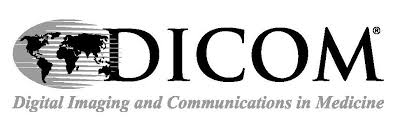
\includegraphics[width=0.7\textwidth]{img/dicom.jpg}
\caption{DICOM}
\end{figure}


DICOM es un protocolo estándar de comunicación entre sistemas de información y a la vez un formato de almacenamiento de imágenes médicas que aparece como solución a los problemas de interoperabilidad entre tipos de dispositivos.

Una imagen médica por sí misma no aporta suficiente información. Para que sea correctamente interpretada es necesario que vaya acompañada de datos del paciente y de la adquisición. Por eso formatos tradicionales como él .jpeg o el .png se quedan cortos.

	El trabajo propuesto parte del interés por aplicar conocimientos del área de ingeniería para brindar soluciones a problemas del área de medicina. En particular
se trabajará en el desarrollo de una solución que ayude a los profesionales de la salud a subir archivos DICOM (Digital Imaging and Communications in Medicine) o imágenes derivadas de estos, y poder previsualizarlos, elegir cuales son de interés, y almacenarlos en un formato estándar.
		DICOM es un estándar reconocido mundialmente para el intercambio de imágenes médicas. Está pensado para el manejo, visualización, almacenamiento, impresión y transmisión de las mismas. Además, incluye la definición de un formato de archivo y de un protocolo de comunicación de red.
		El protocolo de comunicación es un protocolo de aplicación, el cual hace uso del protocolo TCP/IP para comunicarse entre sistemas. Los archivos DICOM
pueden ser compartidos entre dos entidades que sean capaces de recibir imagenes e informacion del paciente en formato DICOM.
		El formato de archivo DICOM tiene la particularidad de tener tanto información de la imagen como información del paciente (metadata). Fue desarrollado con el objetivo de estandarizar el intercambio de imágenes médicas,aún cuando cada fabricante de equipos de imágenes médicas trabaje con su propio enfoque, mientras que formatos como Nifti, Analyze o Minc, apuntan a facilitar y mejorar el análisis de post procesamiento.

		Como se puede observar, es muy importante tener un estándar que se utilice en todos los hospitales para el mismo o similar examen, ya que esto ayuda a evitar problemas como por ejemplo si el paciente se muda de un hospital a otro. DICOM también proporciona interconectividad entre diversos sistemas médicos y soporta
todas las ramas de la medicina, siendo actualmente un estándar exhaustivo. Además DICOM soporta información de imágenes comprimidas, mediante un mecanismo que permite a documentos con distinto formato ser encapsulados y transformados en un archivo DICOM. Los esquemas de compresión soportados por DICOM incluyen los siguientes: JPEG, Run-Length Encoding (RLE), JPEG-LS, JPEG-2000, MPEG2/MPEG4, y Deflated. Un archivo DICOM encapsulado incluye metadata relacionada al documento nativo y además la metadata necesaria para crear la cápsula DICOM.
		La innovación del formato de archivo DICOM fue establecer que la información del píxel no puede ser separada de la descripción del procedimiento
médico que llevó a la formación de la imagen en sí misma. En otras palabras, una imagen que está separada de su metadata se convierte en una imagen médica sin sentido. Metadata y la información del píxel se juntan en un único archivo, y el encabezado DICOM, además de la información sobre la matriz de la imagen, contiene una descripción muy completa sobre el procedimiento utilizado para generar la imagen, además de contener información relevante sobre el paciente. Por todo esto, el encabezado es dependiente de la modalidad de la imagen y varía en tamaño. Esto trae aparejada una desventaja importante que radica en la necesidad de un software especial para poder abrir los archivos DICOM, ya que los distintos sistemas operativos no reconocen este formato de forma nativa [4]. Los visores
		DICOM pueden ser software propietario provisto junto al sistema de imágenes médicas, o de terceros. Dentro de estos últimos, existen herramientas de variado desarrollo, pero con la gran desventaja de que son pagas (RadiAnt, MicroDicom, EMV Dicom Viewer, IrfanView, 3DimViewer) mientras otras requieren de conocimientos técnicos para su implementación y puesta en producción (DICOM Web Viewer, Mango).Otra desventaja que tiene el estándar DICOM está relacionada con los datos de entrada de la información. Esto se debe a la posibilidad de incorporar demasiados campos opcionales al encabezado de un archivo por parte de los
fabricantes de equipos de imágenes médicas. Esta desventaja condujo ainconsistencias en el completado de estos campos. Algunos atributos dentro del encabezado de imágenes DICOM muchas veces están incompletos, se dejan en blanco o completan con información incorrecta. Todo esto es causado por la flexibilidad en la definición de la construcción de los archivos DICOM. El encabezado de un archivo DICOM consiste en un preámbulo y un prefijo, seguido de una secuencia de elementos de datos, El preámbulo contiene bytes reservados que no son utilizados, mientras que el prefijo contiene el texto ASCII “DICM”. Luego del preámbulo y el prefijo viene una secuencia de elementos de datos. Cada uno de ellos consiste en una etiqueta
	DICOM, un código ASCII de dos caracteres indicando el valor de representación, el tamaño del elemento, y el valor. Los elementos de datos en el archivo
estan ordenados por el número de etiqueta DICOM. La imagen en sí misma es solamente otro elemento de datos cuyo valor de representación indica si la información corresponde a una sola imagen, varios cuadros de un estudio o un ciclo de video

\subsection{Caracteristicas del Formato DICOM}
El formato DICOM cuenta con objetos IOD (Information Object Definition), formados por la imagen y su información asociada (Son una representación lógica de objetos del mundo real) y DIMSE (DICOM Message Service Element), operaciones que pueden realizarse sobre un objeto. IOD y DICOM forman SOP, la unidad funcional de DICOM.

Un IOD se compone de IEs (Entidades de información) (Hay IE de paciente, de estudio, de serie,  de equipo, de imagen…) que a su vez se componen de uno o varios módulos que a su vez se contienen varios atributos. Un atributo se define con nombre, etiqueta, tipo y descripción.

\subsection{Composición del estandar DICOM}

\begin{figure}[H]
\centering
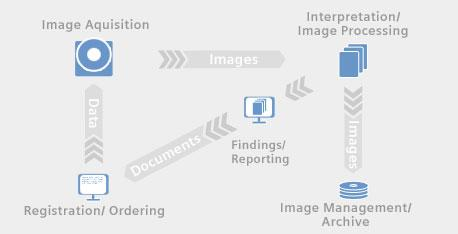
\includegraphics[width=0.7\textwidth]{img/dicom_diagram.jpg}
\caption{Diagrama del proceso para el analisis de imagenes DICOM}
\end{figure}

En el estándar DICOM la información se define mediante un modelo que refleja el mundo real. La imagen es el núcleo de información de un fichero DICOM. Cada fichero contiene, además de la imagen, información sobre el paciente (identificación demográfica y de identificación), el estudio en el que se encuadra la toma de la imagen, la serie a la que pertenece la imagen e información sobre la propia imagen.

\subsection{Importancia del estandar DICOM}

\begin{figure}[H]
\centering
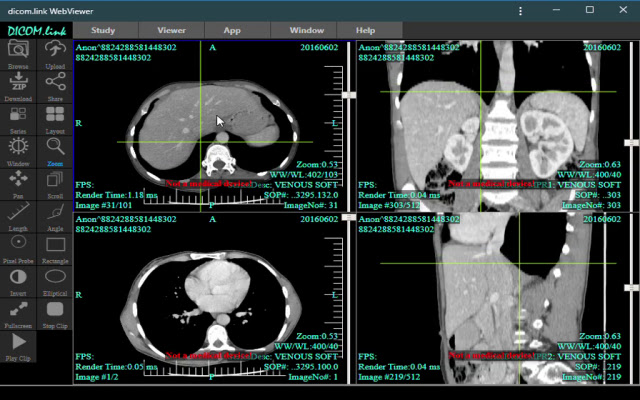
\includegraphics[width=0.7\textwidth]{img/dicom_real.jpg}
\caption{Uso de Software para analizar patologias o anomalias usando DICOM}
\end{figure}

DICOM permite una identificación univoca de objetos. Cada fichero DICOM tiene un UID único compuesto por varios números.

Las comunicaciones DICOM se adaptan al estándar OSI para el intercambio de información. La AE (Entidad de Aplicación) se encarga de las comunicaciones de modo que para cada servicio existe un AE cliente y un AE aplicación.

Gracias a sus características y a su nivel de implantación, hoy día DICOM es mundialmente reconocido para el manejo, almacenamiento, impresión y transmisión de imágenes médicas.

\subsection{Importancia de la Escala Hounsfield}
La escala de Unidades Hounsfield (símbolo HU del inglés ‘Hounsfield Units’) es el resultado de la transformación de la escala de coeficientes de atenuación lineal de rayos X en una nueva escala en la cual el valor de atenuación del agua destilada en Condiciones Normales de Presión y Temperatura (CNPT) se define como 0 unidades de Hounsfield (HU).

En la tomografía computarizada se hace uso de una escala para determinar la densidad de los
tejidos, esta es la escala de unidades Hunsfield(UH), que mediante la atenuación de rayos X se
puede terminar rangos entre -1000 a +1000, cuyos valores dependerá del tejido en cuestión siendo
-1000 un valor dado para la radiosensibilidad del aire , 0 para el agua destilada y +1000 para
tejidos óseos.

\begin{table}[H]
\begin{center}
\begin{tabular}{| c | c |}
\hline
TIPO DE TEJIDO & HU \\ \hline
Hueso compacto & > 250 \\
Hueso esponjoso & 50-300 \\
Sangre coagulada & 70-90 \\
Tiroides & 60-80\\
Hígado & 50-70\\
Sangre entera & 50-60\\
Sustancia gris & 37-41\\
Músculo & 35-50\\
Páncreas & 30-50\\
Riñón & 20-40\\
Sustancia blanca & 20-34\\
Plasma & 27 ± 2\\
LCR & 5-10\\
Grasa & -80 hasta -100\\
Pulmón & -950 hasta -550\\ \hline
\end{tabular}
\end{center}
\end{table}


\section{Metodologia y Desarrollo}

\subsection{Libreria Pydicom}
pydicom es un paquete de Python puro para trabajar con archivos DICOM. Le permite leer, modificar y escribir datos DICOM de una manera fácil y "pitónica".
Como un paquete de Python puro, pydicom puede ejecutarse en cualquier lugar donde se ejecute Python sin ningún otro requisito, aunque si está trabajando con Pixel Data, le recomendamos que también instale NumPy.
\subsection{Lenguaje Utilizado}
\begin{itemize}
	\item Javascript y librerias:
	\item MITK (Medical Imaging Interaction Toolkit)
	\end{itemize}
	


\subsection{Repositorio del Proyecto}

Todo el documento estará alojado en el siguiente Repositorio: https://github.com/AngelYvan/mcc-final-grup5
Para el despliegue de la aplicación se utilizará: 

\subsection{Preparación del entorno de desarrollo}


\begin{itemize}
            \item Software MITK:
\end{itemize}

MITK es un programa de software libre empleado para el análisis de imágenes médicas de
tomografía computerizada. Este programa trabaja con archivos DICOM (Digital Imaging and
Communication in Medicine) que es el formato estándar para el procesamiento de este tipo de
imágenes. En ella se puede encontrar versiones actualizadas del programa así como un manual para el usuario con explicaciones de las herramientas de las que dispone y otro manual para desarrolladores.

En el diseño del código se ha trabajado contando con las librerías “Medical Imaging Interaction Toolkit (MITK) debido a la facididad para el manejo de las imagenes en formatp DIVOM que se están utilizando.

\begin{figure}[H]
\centering
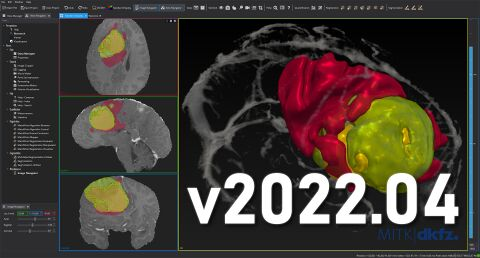
\includegraphics[width=0.7\textwidth]{img/MITK.jpg}
\caption{Software MITK}
\end{figure}

\subsection{Procesamiento de la Imagen}

Se tendrá una base de datos con imagenes de tomografía con 3 vistas (Superior, Frontal y Lateral). Donde el algoritmo KDTree hará un analisis de puntos para determinar las patologias preexistentes en el paciente.

\subsection{Utilizando el Algoritmo KDTree}
\subsection{Output: Detectando las patologias}




	\section{Resultados}
	\begin{itemize}
		\item Se logró aplicar  un algoritmo computacional para la detección de patologias en imagenes DICOM
		\item Se determinó la presencia de patologias en imagenes DICOM mediante el uso de algoritmos computacionales y basados en la escala Hounsfield
		\end{itemize}
		


	\section{Conclusiones}


	
	
\end{document}
